% !TeX spellcheck = en_US

%TODO Sibel

\begin{comment}
- data obtained from an earlier human-subject study
\end{comment}

\begin{frame}{Setup}
	\begin{itemize}
		\item \Highlight{\textbf{2}} geometrically distinct placements of the line for each of the \Highlight{\textbf{19}} topologically distinct relations %\Highlight{$\implies$}
		
		\item a total of \Highlight{\textbf{38}} diagrams each showing a line and a region
		
		\item line \Highlight{$\rightarrow$} road, region \Highlight{$\rightarrow$} park
		
		\item parks in all diagrams same size and shape
		
		\item 28 participants
	\end{itemize}
\end{frame}

\begin{frame}{Setup (cont.)}
	\only<1>
	{
		\begin{center}
			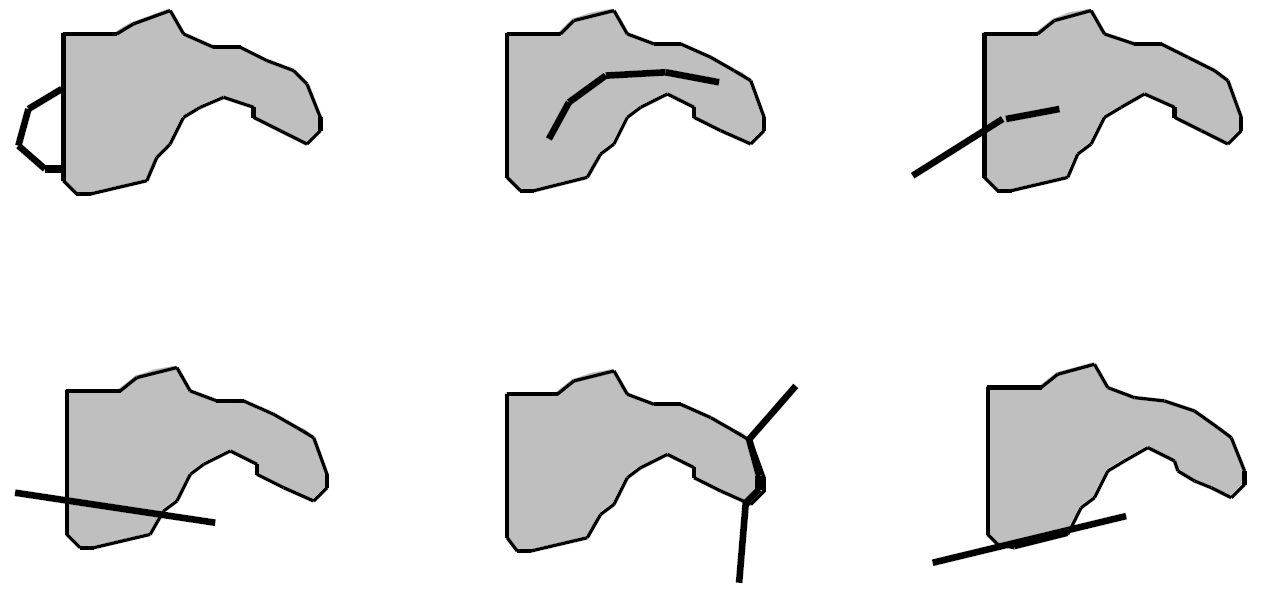
\includegraphics[width=\textwidth]{images/evaluation_setup.png}
		\end{center}
		\begin{tabularx}{\textwidth}{c X}
			\Highlight{\textbf{Q:}} & Find the pair that is topologically identical from among all geometrically distinct diagrams. \\
			 & \\
		\end{tabularx}
		%Here are six of the diagrams that were used in this research, which are obviously all geometrically distinct. 
	}
	
	\only<2>
	{
		\begin{center}
			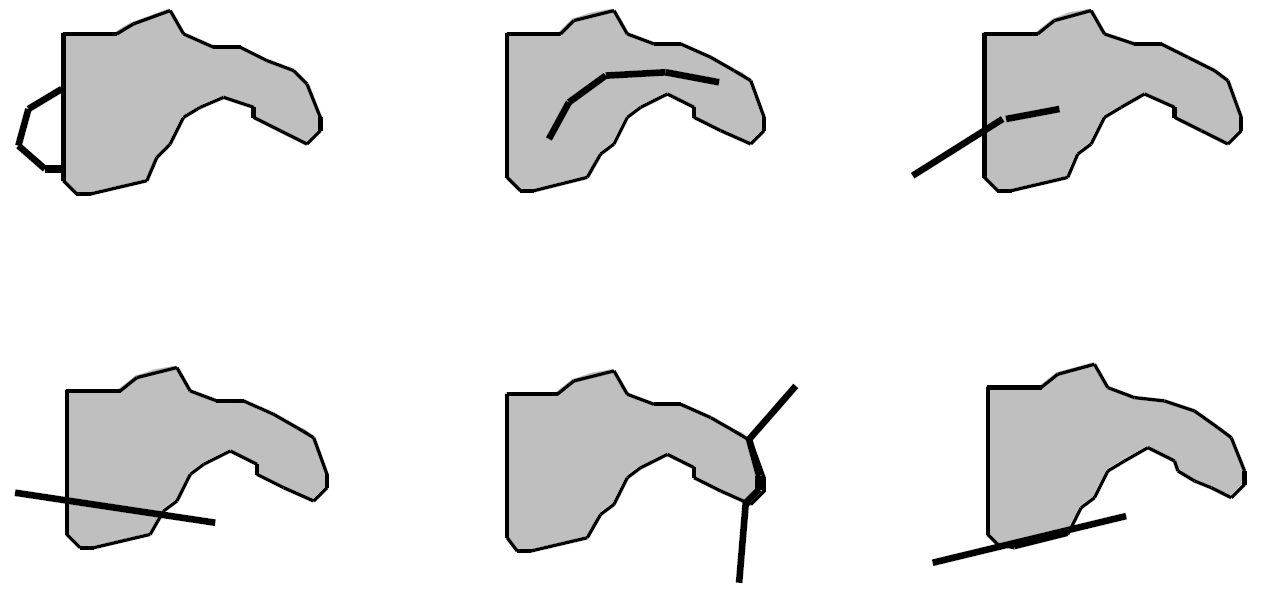
\includegraphics[width=\textwidth]{images/evaluation_setup.png}
		\end{center}
		\begin{tabularx}{\textwidth}{c X}
			\Highlight{\textbf{Q:}} & Find the pair that is topologically identical from among all geometrically distinct diagrams. \\
			\Highlight{\textbf{A:}} & The right and middle examples in the lower row. \\
		\end{tabularx}
	}
\end{frame}
\begin{comment}
	- some examples of the stimuli used in this research. The right and middle examples in the lower row are topologically identical but geometrically-distinct.
\end{comment}

\begin{frame}{Task}
	\begin{itemize}
		%\item group spatial relations between line and region, road and park (parks were all the same size and shape)
		\item arrange the sketches into several groups, such that you would use the same verbal description for the spatial relationship between the road and the park for every sketch in each group
	\end{itemize}
\end{frame}

\begin{frame}{Goal}
	\begin{block}{Goal}
		\begin{itemize}
			\item analyse how the subjects formed groups of similar relations
			\item check similarity with presented conceptual neighborhood models
		\end{itemize}
	\end{block}
\end{frame}

\begin{frame}{Results}
	\begin{block}{ }
	Each spatial relation could be grouped as many as 112 times (4 pairs times 28 subjects) with each other relation.
	\end{block}
	\begin{block}{Number of times conceptual neighbors are grouped:}
		%The number of times subjects grouped pairs of relations that are conceptual neighbors in the snapshot model only, the smooth-transition model only, in both models, and in neither model.
		\begin{center}
			\begin{tabular}{|l|c|rrrr|}
				\hline
				 & \dots\footnote{Number of relations that are conceptual neighbors} & \multicolumn{1}{c}{\textit{min}} & \multicolumn{1}{c}{\textit{max}} & \multicolumn{1}{c}{\textit{mean}} & \multicolumn{1}{c|}{\textit{\%}\footnote{percentage = mean / 112}} \\
				\hline
				snapshot model only & 2 & 10 & 16 & 13.0 & 11.6 \\
				% The two pairs that were snapshot neighbours - but not smooth transition neighbours - were grouped 10 and 16 times (mean =13; 11.6 %).
				smooth-transition model only & 12 & 0 & 66 & 17.3 & 15.4 \\
				% Those pairs that were neighbours for smooth transitions - but not snapshots - were grouped between 0 and 66 times, with a mean of 17.3 (15.4 %).
				both models & 26 & 0 & 78 & 33.6 & 29.5 \\
				% The pairs that were neighbours by both snapshot and smooth-transiiton models were grouped from 0 to 78 times, with a mean of 33.6.
				neither model & 131 & - & - & 6.0 & 5.3 \\
				% Perhaps most significant, however, is the fact that the 131 pairs that were neighbors by neither the snapshot model nor the smooth transitions were grouped an average of only 6.0 times by the subject (5.3 per cent of the maximum).
				%Sixty pairs were never grouped by any of the 28 subjects nor any of the four possible stimulus pairs. The most frequently-grouped pair in this category was 54 times (48 per cent), but only 20 stimulus pairs with neither smooth transitions nor minimum snapshot difference were grouped 12 or more times (10 per cent of the maximum).
				\hline
			\end{tabular}
		\end{center}
	\end{block}
\end{frame}

\begin{comment}
	%		\item Goal: Within the context of different models for conceptual neighbors, it is particularly enlightening to analyse how the subjects formed groups of similar relations.'
	%		
	%		\item 28 subjects performing tasks
	%		
	%		\item each spatial relation could be grouped as many as 112 times (4 pairs times 28 subjects) with each other relation
	%	\end{itemize}
\end{comment}
